%!TEX root = ../rules-working.tex
%LTeX: enabled=false

\silentlychangedin{1B}{1B-figures}{

\begin{onecolumnfigure}[h!]

{\bfseries Example of Lateral Toss Attack}

\includegraphics[width=\linewidth]{figures/figure-lateral-toss-bombing-example.pdf}

\end{onecolumnfigure}

}{

\begin{onecolumnfigure}

\begin{fitheight}{8.2\standardhexwidth}
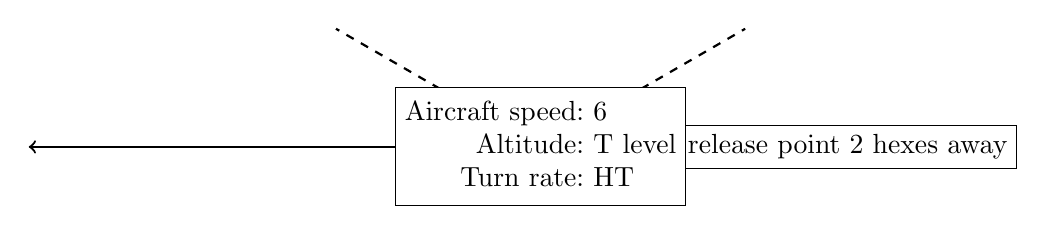
\begin{tikzpicture}

    \setfiguresize{-5.5}{-4.1}{+5.5}{4.1}

    \drawevenhexgrid{-5}{-3.5}{11}{8}  

    
    \begin{scope}[thick,dashed]
        \miniathex{+0.00}{0.00}{\draw (30:0.0) -- (30:3.0);}
        \miniathex{-2.00}{0.00}{\draw (150:0.0) -- (150:3.0);}
    \end{scope}
    \begin{scope}[thick,->]
        \miniathex{+4.00}{0.00}{\draw (180:0.0) -- (180:6.5);}
    \end{scope}
    \miniathex{-2.20}{0.20}{\node [anchor=west] {X};}

    \miniathex{-2.20}{-2.00}{\node [anchor=west,fill=white,draw] {X = bomb release point 2 hexes away};}
    \miniathex{-4.00}{-1.00}{\node [fill=white,draw] {Target};}
    \miniathex{+3.00}{-0.50}{\node [fill=white,draw] {Line-of-Approach};}
    \miniathex{+3.00}{+2.50}{\node [fill=white,draw] {\begin{tabular}{@{}r@{ }l@{}}Aircraft speed:&6\\Altitude:&T level\\Turn rate:&HT\\\end{tabular}};}

    \drawaircraftcounter{+2.00}{+1.00}{210}{F-105}{}{}
    \drawaircraftcounter{-3.00}{+0.50}{150}{F-105}{}{}
    \drawgroundunitcounter{-4.00}{+0.00}{90}{}{}

\end{tikzpicture}
\end{fitheight}

\figurecaption{figure:lateral-toss-bombing-example}{Lateral Toss Bombing Example.}

\end{onecolumnfigure}

}
